% TODO
\hbox{}
\vskip-12mm
\hbox{}

\section{Experimental Apparatus}
\label{sec:exp apparatus}

\begin{figure*}
\begin{center}
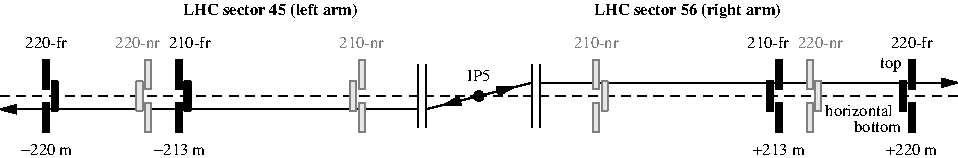
\includegraphics{fig/elastic_principle.pdf}
\caption{%
Schematic view of the RP units used for the presented measurement (black squares) with two proton tracks from an elastic event (lines with arrows). The numbers at the bottom indicate the distance from the interaction point (IP5).
}
% TODO
\vskip-6mm
\label{fig:rpsketch}
\end{center}
\end{figure*}

The TOTEM experiment, located at the LHC Interaction Point (IP) 5 together with the CMS experiment, is dedicated to the measurement of the total cross-section, elastic scattering and diffractive processes. The experimental apparatus, symmetric with respect to the IP, detects particles at different scattering angles in the forward region: a forward proton spectrometer composed of detectors in Roman Pots (RPs) and the magnetic elements of the LHC and, to measure at larger angles, the forward tracking telescopes T1 and T2. A complete description of the TOTEM detector instrumentation and its performance is given in~\cite{totem-jinst} and~\cite{totem-ijmp}. The data analysed here come from the RPs only. 

A RP is a movable beam-pipe insertion which houses the tracking detectors that are thus capable of approaching the LHC beam to a distance of less than a millimetre, and to detect protons with scattering angles of only a few microradians. The proton spectrometer is organised in two arms: one on the left side of the IP (LHC sector 45) and one on the right (LHC sector 56), see Figure~\ref{fig:rpsketch}. In each arm, there are several RP units. The presented measurement is performed with units ``210-fr'' (approximately $213\un{m}$ from the IP) and ``220-fr'' (about $220\un{m}$ from the IP). The 210-fr unit is tilted by $8^\circ$ in the transverse plane with respect to the 220-fr unit. Each unit consists of 3 RPs, one approaching the outgoing beam from the top, one from the bottom, and one horizontally. Each RP houses a stack of 5 ``U'' and 5 ``V'' silicon strip detectors, where ``U'' and ``V'' refer to two mutually perpendicular strip orientations. The special design of the sensors is such that the insensitive area at the edge facing the beam is only a few tens of micrometres \cite{edgeless-strips}. Due to the $7\un{m}$ long lever arm between the two RP units in one arm, the local track angles can be reconstructed with an accuracy  of about $2.5\un{\mu rad}$.

Since elastic scattering events consist of two collinear protons emitted in opposite directions, the detected events can have two topologies, called ``diagonals'': 45 bottom -- 56 top and 45 top -- 56 bottom, where the numbers refer to the LHC sector.

This article uses a reference frame where $x$ denotes the horizontal axis (pointing out of the LHC ring), $y$ the vertical axis (pointing against gravity) and $z$ the beam axis (in the clockwise direction).
